%
% slides.tex -- Slides zur THC
%
% (c) 2017 Prof Dr Andreas Müller, Hochschule Rapperswil
%
\theoremstyle{definition}
\newtheorem{aufgaben}{Aufgaben}
\newtheorem{temperatur}{Temperaturabhängigkeit der Dichte}
\newtheorem{salinity}{Salzgehalt und Dichte}

\begin{document}

\ifthenelse{\boolean{presentation}}{

\subtitle{\strut}

\begin{frame}
\titlepage
\end{frame}

\subtitle{\strut Golfstrom}

\begin{frame}
\titlepage
\end{frame}

}{}

\begin{frame}
\frametitle{Förderband}
\begin{center}
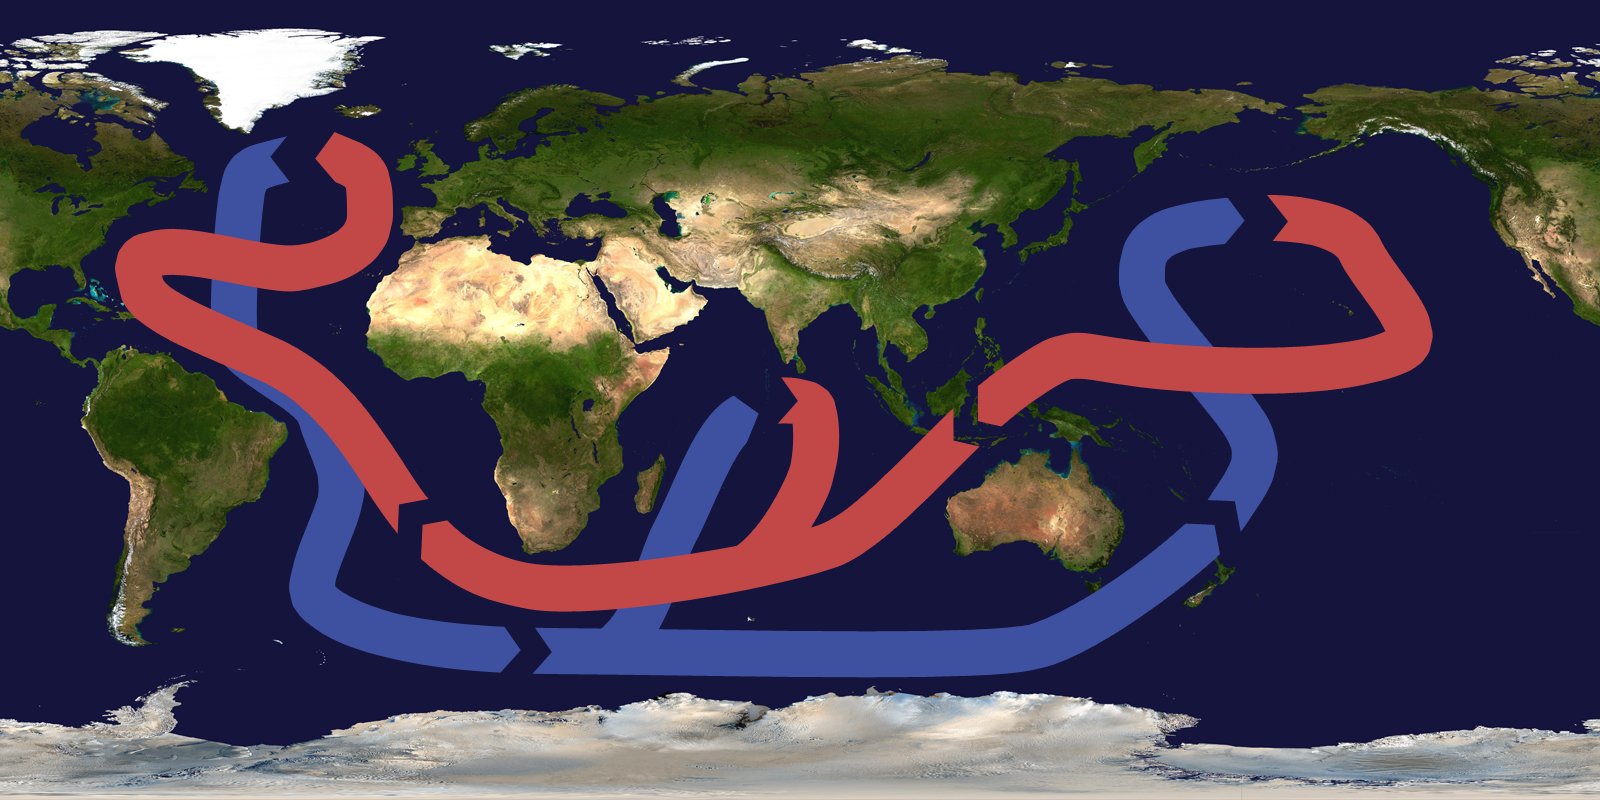
\includegraphics[width=\hsize]{Thermohaline_circulation.png}
\end{center}
\end{frame}

\begin{frame}
\frametitle{Thermohaline Zirkulation}
\begin{definition}
Die {\em thermohaline Zirkulation} ist die
globale Umwälzung der Weltmeere angetrieben von Dichteunterschieden
verursacht durch Unterschiede in Temperatur und Salzgehalt.
\end{definition}

\begin{aufgaben}
\begin{itemize}
\item Abgestorbenes Plankton sinkt in die Tiefe
\item THC transportiert Nährstoffe wieder nach oben
\item Energietransport vom Äquator in höhere Breiten
(Golfstrom)
\end{itemize}
\end{aufgaben}

\end{frame}

\begin{frame}
\frametitle{Dichte von Wasser}
\begin{temperatur}
\begin{itemize}
\item
Kaltes Wasser hat höhere Dichte als warmes Wasser 
\item
Dichteanomalie von Süsswasser (maximale Dichte bei $4^\circ\text{C}$)
verschwindet bei höherem Salzgehalt
\end{itemize}
\end{temperatur}

\begin{salinity}
\begin{itemize}
\item Einheit: g Salz pro kg Meerwasser
\item Messmethode heute: elektrische Leitfähigkeit steigt mit der Salinität,
PSU (practical salinity unit, PSS-78 practical salinity scale)
\item typischer Wert: $35$
\item Höherer Salzgehalt bedeutet höhere Dichte
\item Gefrieren: Wasser mit höherer Salinität bleibt zurück
\end{itemize}
\end{salinity}

\end{frame}

\begin{frame}
\frametitle{Box-Modell}
\begin{center}
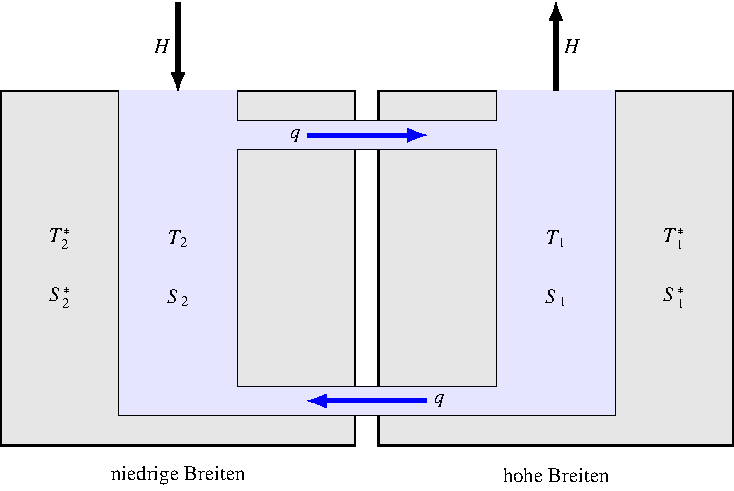
\includegraphics[width=0.8\hsize]{../../skript/chapters/4/boxmodell.pdf}
\end{center}
\end{frame}

\end{document}
